\documentclass[12pt,a4paper]{scrartcl}
\usepackage[utf8]{inputenc}
\usepackage[english,russian]{babel}
\usepackage{indentfirst}
\usepackage{misccorr}
\usepackage{graphicx}
\usepackage{amsmath}
\usepackage{multirow}
\usepackage{pgfplots}
\usepackage{parskip}
\usepackage[top=1cm, bottom=1cm, left=1cm, right=1cm]{geometry}
\pgfplotsset{compat=1.9}

\begin{document}
	\graphicspath{{/home/cd7567/Pictures/TeXImgs}}
	
	\newcommand{\ms}{\mathstrut}
	\newcommand{\msp}{\hspace{0.5cm}}
	\newcommand{\al}{\alpha}
	\newcommand{\dg}{^\circ}
	\newcommand{\dif}{\mathrm{d}}
	\newcommand{\qd}[2]{^{\frac{#1}{#2}}}
	\newcommand{\qdm}[2]{^{-\frac{#1}{#2}}}
	\newcommand{\lm}[2]{\underset{#1 \rightarrow #2}{\lim}}
	\newcommand{\sfrac}[2]{\dfrac{\strut #1}{\strut #2}}
	\newcommand{\equal}[1]{\overset{(#1)}{=}}
	\newcommand{\linevdots}{\ \raisebox{-.08\height}{\vdots}\ }
	\newcommand{\linecvdots}{\ \raisebox{-.08\height}{\vdots}\hspace{-0.13cm}\raisebox{.15\height}{\cancel{\phantom{a}}\hspace{0.06cm}}}
	\newcommand{\combox}[1]{\ms \msp \msp \begin{minipage}{0.95\linewidth}
			#1
	\end{minipage}}
	
	\newtheorem{pr}{Задача}
	\newtheorem{ex}{Пример}
	\newtheorem{dfn}{Def}
	\newtheorem{theorem}{Th}
	
	\newenvironment{slv}{\ms \msp \textit{Решение:}}{}
	\newenvironment{proof}{\ms \msp \textit{Доказательство: }}{\hfill $\square$}
	
	\begin{titlepage}
		
		\vspace*{\fill}
		
		\begin{center}
			
\includegraphics[scale=0.8]{MIPT.png}
			\\[0.7cm]\Huge Московский Физико-Технический Институт\\(национальный исследовательский университет)
			\\[2cm]\LARGE Отчет по эксперименту
			\\[0.5cm]\noindent\rule{\textwidth}{1pt}
			\\\Huge\textbf{Измерение удельной теплоемкости воздуха\\при постоянном давлении}
			\\[-0.5cm]\noindent\rule{\textwidth}{1pt}
		\end{center}
		
		\begin{flushleft}
			\textit{Работа №2.1.1; дата: 18.03.22}\hfill\textit{Семестр: 2}
		\end{flushleft}
		
		\vspace*{\fill}
		
		\begin{flushleft}
			Выполнил: \hspace{\fill} Группа:
			\\Кошелев Александр \hspace{\fill} Б05-105
		\end{flushleft}
	\end{titlepage}
	
	%Страница 2
	
	\begin{flushleft}
		\footnotesize{Измерение удельной теплоемкости воздуха при постоянном давлении} \hspace{\fill} \footnotesize{2}
		\\[-0.3cm]\noindent\rule{\textwidth}{0.3pt}
	\end{flushleft}
	
	\section{Аннотация}
	
	\textbf{Цель работы: }
	
	Измерить повышение температуры воздуха в зависимости от мощности подводимого
	тепла и расхода при стационарном течении через трубу; исключив тепловые потери, по результатам
	измерений определить теплоёмкость воздуха при постоянном давлении.
	
	\textbf{Схема установки:}
	\begin{center}
		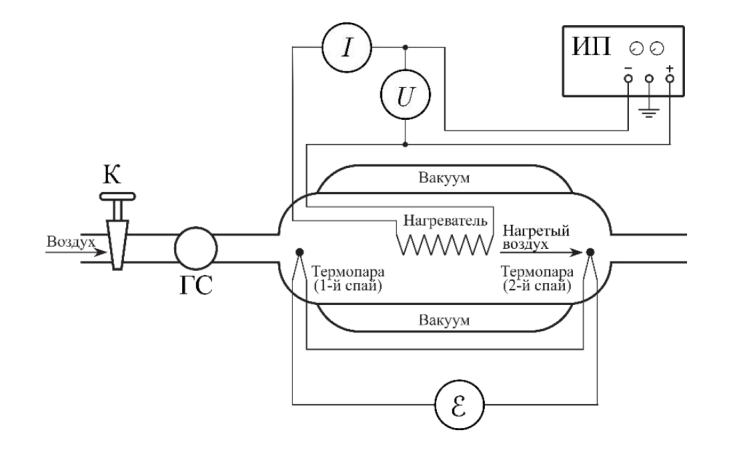
\includegraphics[scale=0.3]{PIC_1.png}
		\\\textbf{Рис. 1:} Схема установки
	\end{center}
		
	\textbf{В работе используются:}
	
	Теплоизолированная стеклянная трубка; электронагреватель; источник питания постоянного тока; амперметр, вольтметр (цифровые мультиметры); термопара, подключенная к микровольтметру; компрессор; газовый счётчик; секундомер.
	
	\section{Теоретические сведения}
	Из курса термодинамики известно уравнение Менделеева-Клапейрона:
	$$PV = \nu RT$$
	Откуда легко выражается плотность воздуха:
	$$\rho = \sfrac{\mu P}{RT}$$
	Также нам понадобится определение массового расхода воздуха:
	$$q = \rho \sfrac{\dif V}{\dif T}$$
	Теперь про условия проведения опыта: давление постоянно, и перепад температур мал, поэтому удельную теплоемкость воздуха можно считать постоянной. В этом случае с учетом закона Ньютона-Рихмана выражение для мощности принимает вид:
	$$N = (c_p q + \alpha)\Delta T$$
	где $\alpha$ - некоторая константа. То есть, зависимость подводимой мощности от разности температур линейна.
	
	\newpage 
	
	%Страница 3
	
	\begin{flushleft}
		\footnotesize{Измерение удельной теплоемкости воздуха при постоянном давлении} \hspace{\fill} \footnotesize{3}
		\\[-0.3cm]\noindent\rule{\textwidth}{0.3pt}
	\end{flushleft}

	\section{Проведение эксперимента}
	\paragraph{Основные параметры при проведении эксперимента} \hfill
	
	Основные параметры среды были замерены напрямую, и легче всего представимы в табличной форме:
	
	\begin{center}
		\begin{tabular}{|c|c|c|}
			\hline
			$P_0$, мм.рт.ст & $T_0$, К & $\rho$, кг/м$^3$
			\\\hline
			$744.6 \pm 0.1$ & $296.2 \pm 0.2$ & $1.192 \pm 0.001$
			\\\hline
		\end{tabular}
		\\\textbf{Табл. 1:} Основные параметры эксперимента
	\end{center}

	\paragraph{Проведение опыта с полностью открытым вентилем подачи} \hfill
	
	Приведем результаты измерения расхода в табличном виде:
	\begin{center}
		\begin{tabular}{|c|c|c|c|c|c|}
			\hline
			$i$, номер & 1 & 2 & 3 & 4 & 5
			\\\hline
			$\Delta V$, л & 5 & 5 & 5 & 5 & 5
			\\\hline
			$\Delta t$, с & $25.20 \pm 0.10$ & $25.34 \pm 0.10$ & $25.10 \pm 0.10$ & $25.31 \pm 0.10$ & $25.16 \pm 0.10$
			\\\hline
			$q$, л/с & $0.1984 \pm 0.0008$ & $0.1973 \pm 0.0008$ & $0.1992 \pm 0.0008$ & $0.1976 \pm 0.0008$ & $0.1987 \pm 0.0008$
			\\\hline
			$\overline{q}$, л/с & \multicolumn{5}{|c|}{$0.1982 \pm 0.0008$}
			\\\hline 
		\end{tabular}
		\\\textbf{Табл. 2:} Расход воздуха в первом опыте
	\end{center}

	Теперь проведем сам эксперимент. Результаты также в табличном виде:
	\begin{center}
		\begin{tabular}{|c|c|c|c|c|c|}
			\hline
			i, номер & $\varepsilon$, мВ & $\Delta T$, К & $I$, мА & $U$, В & $N$, мВ
			\\\hline
			1 & $0.038 \pm 0.001$ & $0.934 \pm 0.025$ & $86.93 \pm 0.01$ & $3.09 \pm 0.01$ & $268.6 \pm 0.9$
			\\\hline
			2 & $0.070 \pm 0.001$ & $1.720 \pm 0.025$ & $115.45 \pm 0.01$ & $4.07 \pm 0.01$ & $469.9 \pm 1.2$
			\\\hline
			3 & $0.090 \pm 0.001$ & $2.211 \pm 0.025$ & $128.08 \pm 0.01$ & $4.52 \pm 0.01$ & $578.9 \pm 1.3$
			\\\hline
			4 & $0.107 \pm 0.001$ & $2.629 \pm 0.025$ & $143.48 \pm 0.01$ & $5.06 \pm 0.01$ & $726.0 \pm 1.4$
			\\\hline
			5 & $0.124 \pm 0.001$ & $3.047 \pm 0.025$ & $153.26 \pm 0.01$ & $5.42 \pm 0.01$ & $830.7 \pm 1.5$
			\\\hline
			6 & $0.147 \pm 0.001$ & $3.612 \pm 0.025$ & $169.92 \pm 0.01$ & $5.99 \pm 0.01$ & $1017 \pm 1.7$
			\\\hline
			7 & $0.191 \pm 0.001$ & $4.693 \pm 0.025$ & $191.11 \pm 0.01$ & $6.74 \pm 0.01$ & $1288 \pm 1.9$
			\\\hline
 		\end{tabular}
 		\\\textbf{Табл. 3:} Проведение эксперимента
	\end{center}

	Построим график зависимости $N(\Delta T)$ и рассчитаем $\gamma_1$ - коэффициент наклона.
	
	\begin{center}
		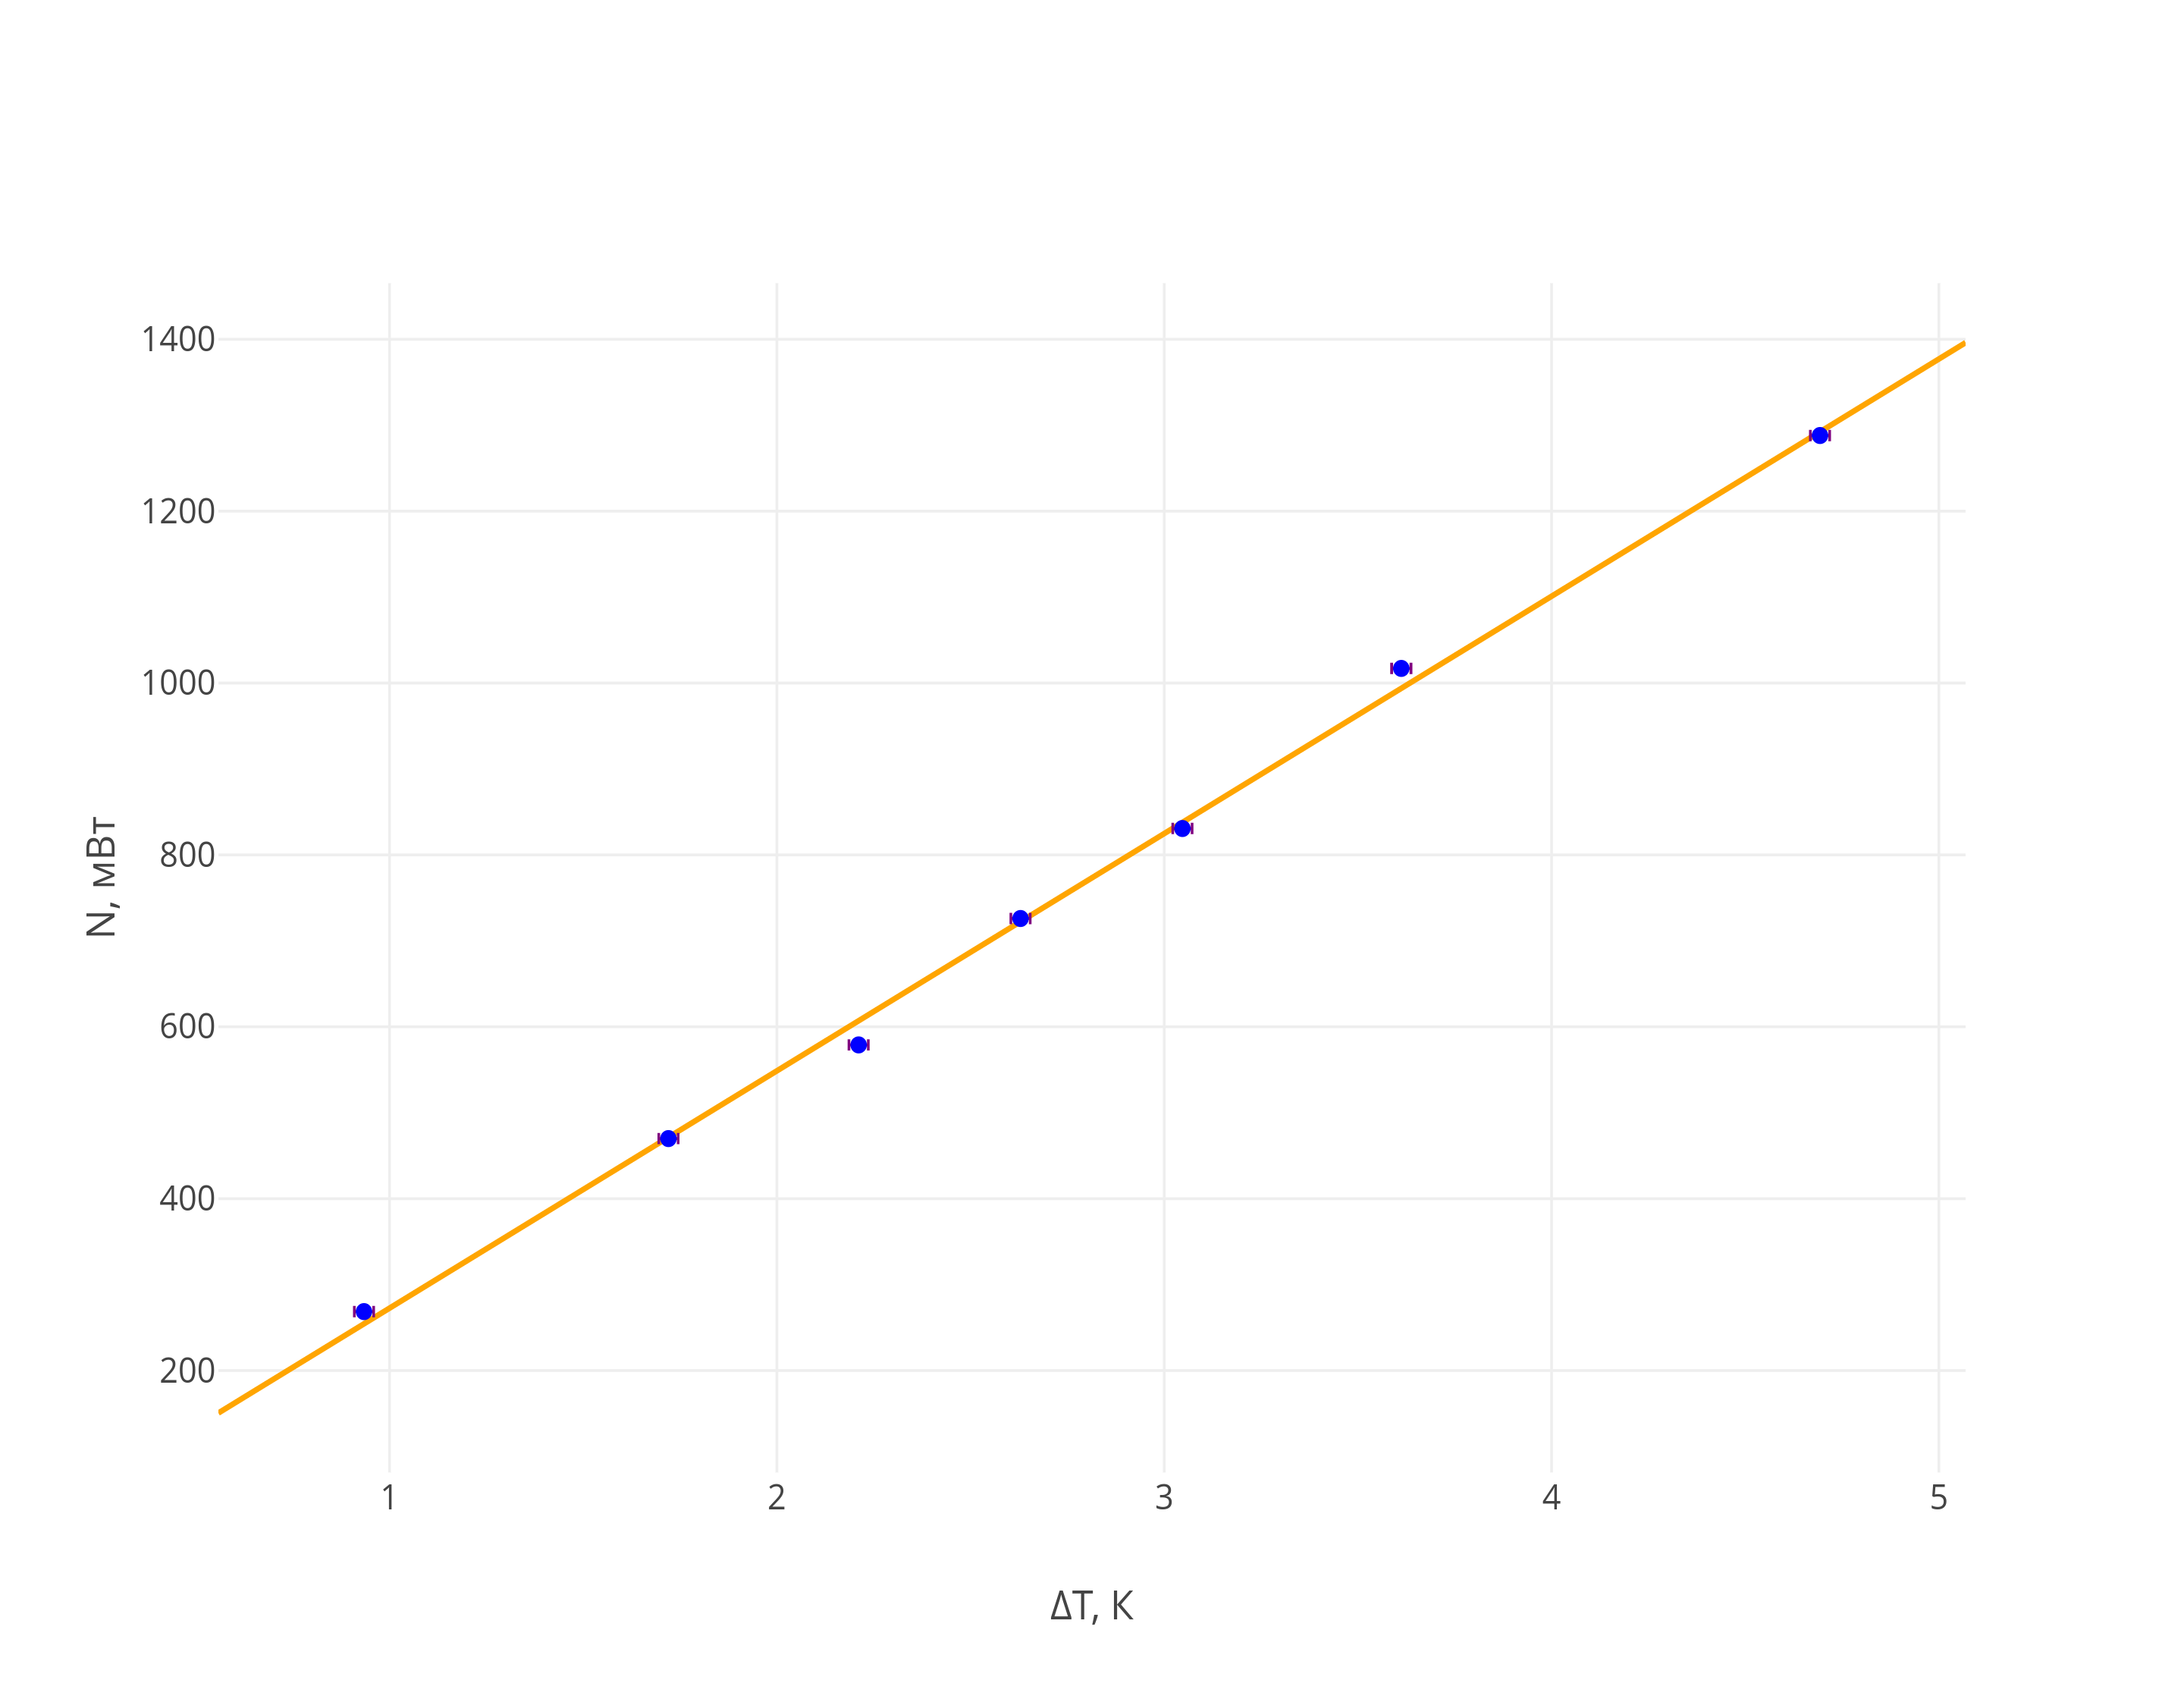
\includegraphics[scale=0.112]{PIC_2.png}
		\\\textbf{Рис. 2:} График зависимости $N(\Delta T)$
	\end{center}

	\newpage
	
	%Страница 4
	
	\begin{flushleft}
		\footnotesize{Измерение удельной теплоемкости воздуха при постоянном давлении} \hspace{\fill} \footnotesize{4}
		\\[-0.3cm]\noindent\rule{\textwidth}{0.3pt}
	\end{flushleft}
	
	$$\gamma_1 = 276 \pm 12\ \text{мВт}/\text{К}$$
	
	\paragraph{Проведение опыта с полуоткрытым вентилем подачи} \hfill
	
	Приведем результаты измерения расхода в табличном виде:
	\begin{center}
		\begin{tabular}{|c|c|c|c|c|c|}
			\hline
			$i$, номер & 1 & 2 & 3 & 4 & 5
			\\\hline
			$\Delta V$, л & 5 & 5 & 5 & 5 & 5
			\\\hline
			$\Delta t$, с & $37.25 \pm 0.10$ & $36.95 \pm 0.10$ & $37.17 \pm 0.10$ & $37.15 \pm 0.10$ & $36.98 \pm 0.10$
			\\\hline
			$q$, л/с & $0.1342 \pm 0.0004$ & $0.1353 \pm 0.0004$ & $0.1345 \pm 0.0004$ & $0.1346 \pm 0.0004$ & $0.1352 \pm 0.0004$
			\\\hline
			$\overline{q}$, л/с & \multicolumn{5}{|c|}{$0.1348 \pm 0.0004$}
			\\\hline 
		\end{tabular}
		\\\textbf{Табл. 4:} Расход воздуха во втором опыте
	\end{center}
	
	Теперь проведем сам эксперимент. Результаты также в табличном виде:
	\begin{center}
		\begin{tabular}{|c|c|c|c|c|c|}
			\hline
			i, номер & $\varepsilon$, мВ & $\Delta T$, К & $I$, мА & $U$, В & $N$, мВ
			\\\hline
			1 & $0.054 \pm 0.001$ & $1.335 \pm 0.025$ & $87.27 \pm 0.01$ & $3.08 \pm 0.01$ & $268.6 \pm 0.9$
			\\\hline
			2 & $0.079 \pm 0.001$ & $1.947 \pm 0.025$ & $103.55 \pm 0.01$ & $3.76 \pm 0.01$ & $389.3 \pm 1.0$
			\\\hline
			3 & $0.096 \pm 0.001$ & $2.359 \pm 0.025$ & $117.27 \pm 0.01$ & $4.01 \pm 0.01$ & $470.3 \pm 1.2$
			\\\hline
			4 & $0.123 \pm 0.001$ & $3.028 \pm 0.025$ & $131.47 \pm 0.01$ & $4.63 \pm 0.01$ & $608.7 \pm 1.3$
			\\\hline
			5 & $0.153 \pm 0.001$ & $3.750 \pm 0.025$ & $145.60 \pm 0.01$ & $5.13 \pm 0.01$ & $746.9 \pm 1.5$
			\\\hline
			6 & $0.183 \pm 0.001$ & $4.503 \pm 0.025$ & $159.78 \pm 0.01$ & $5.63 \pm 0.01$ & $899.6 \pm 1.6$
			\\\hline
			7 & $0.214 \pm 0.001$ & $5.262 \pm 0.025$ & $172.11 \pm 0.01$ & $6.07 \pm 0.01$ & $1045 \pm 1.7$
			\\\hline
		\end{tabular}
		\\\textbf{Табл. 5:} Проведение эксперимента
	\end{center}
	
	Построим график зависимости $N(\Delta T)$ и рассчитаем $\gamma_1$ - коэффициент наклона.
	
	\begin{center}
		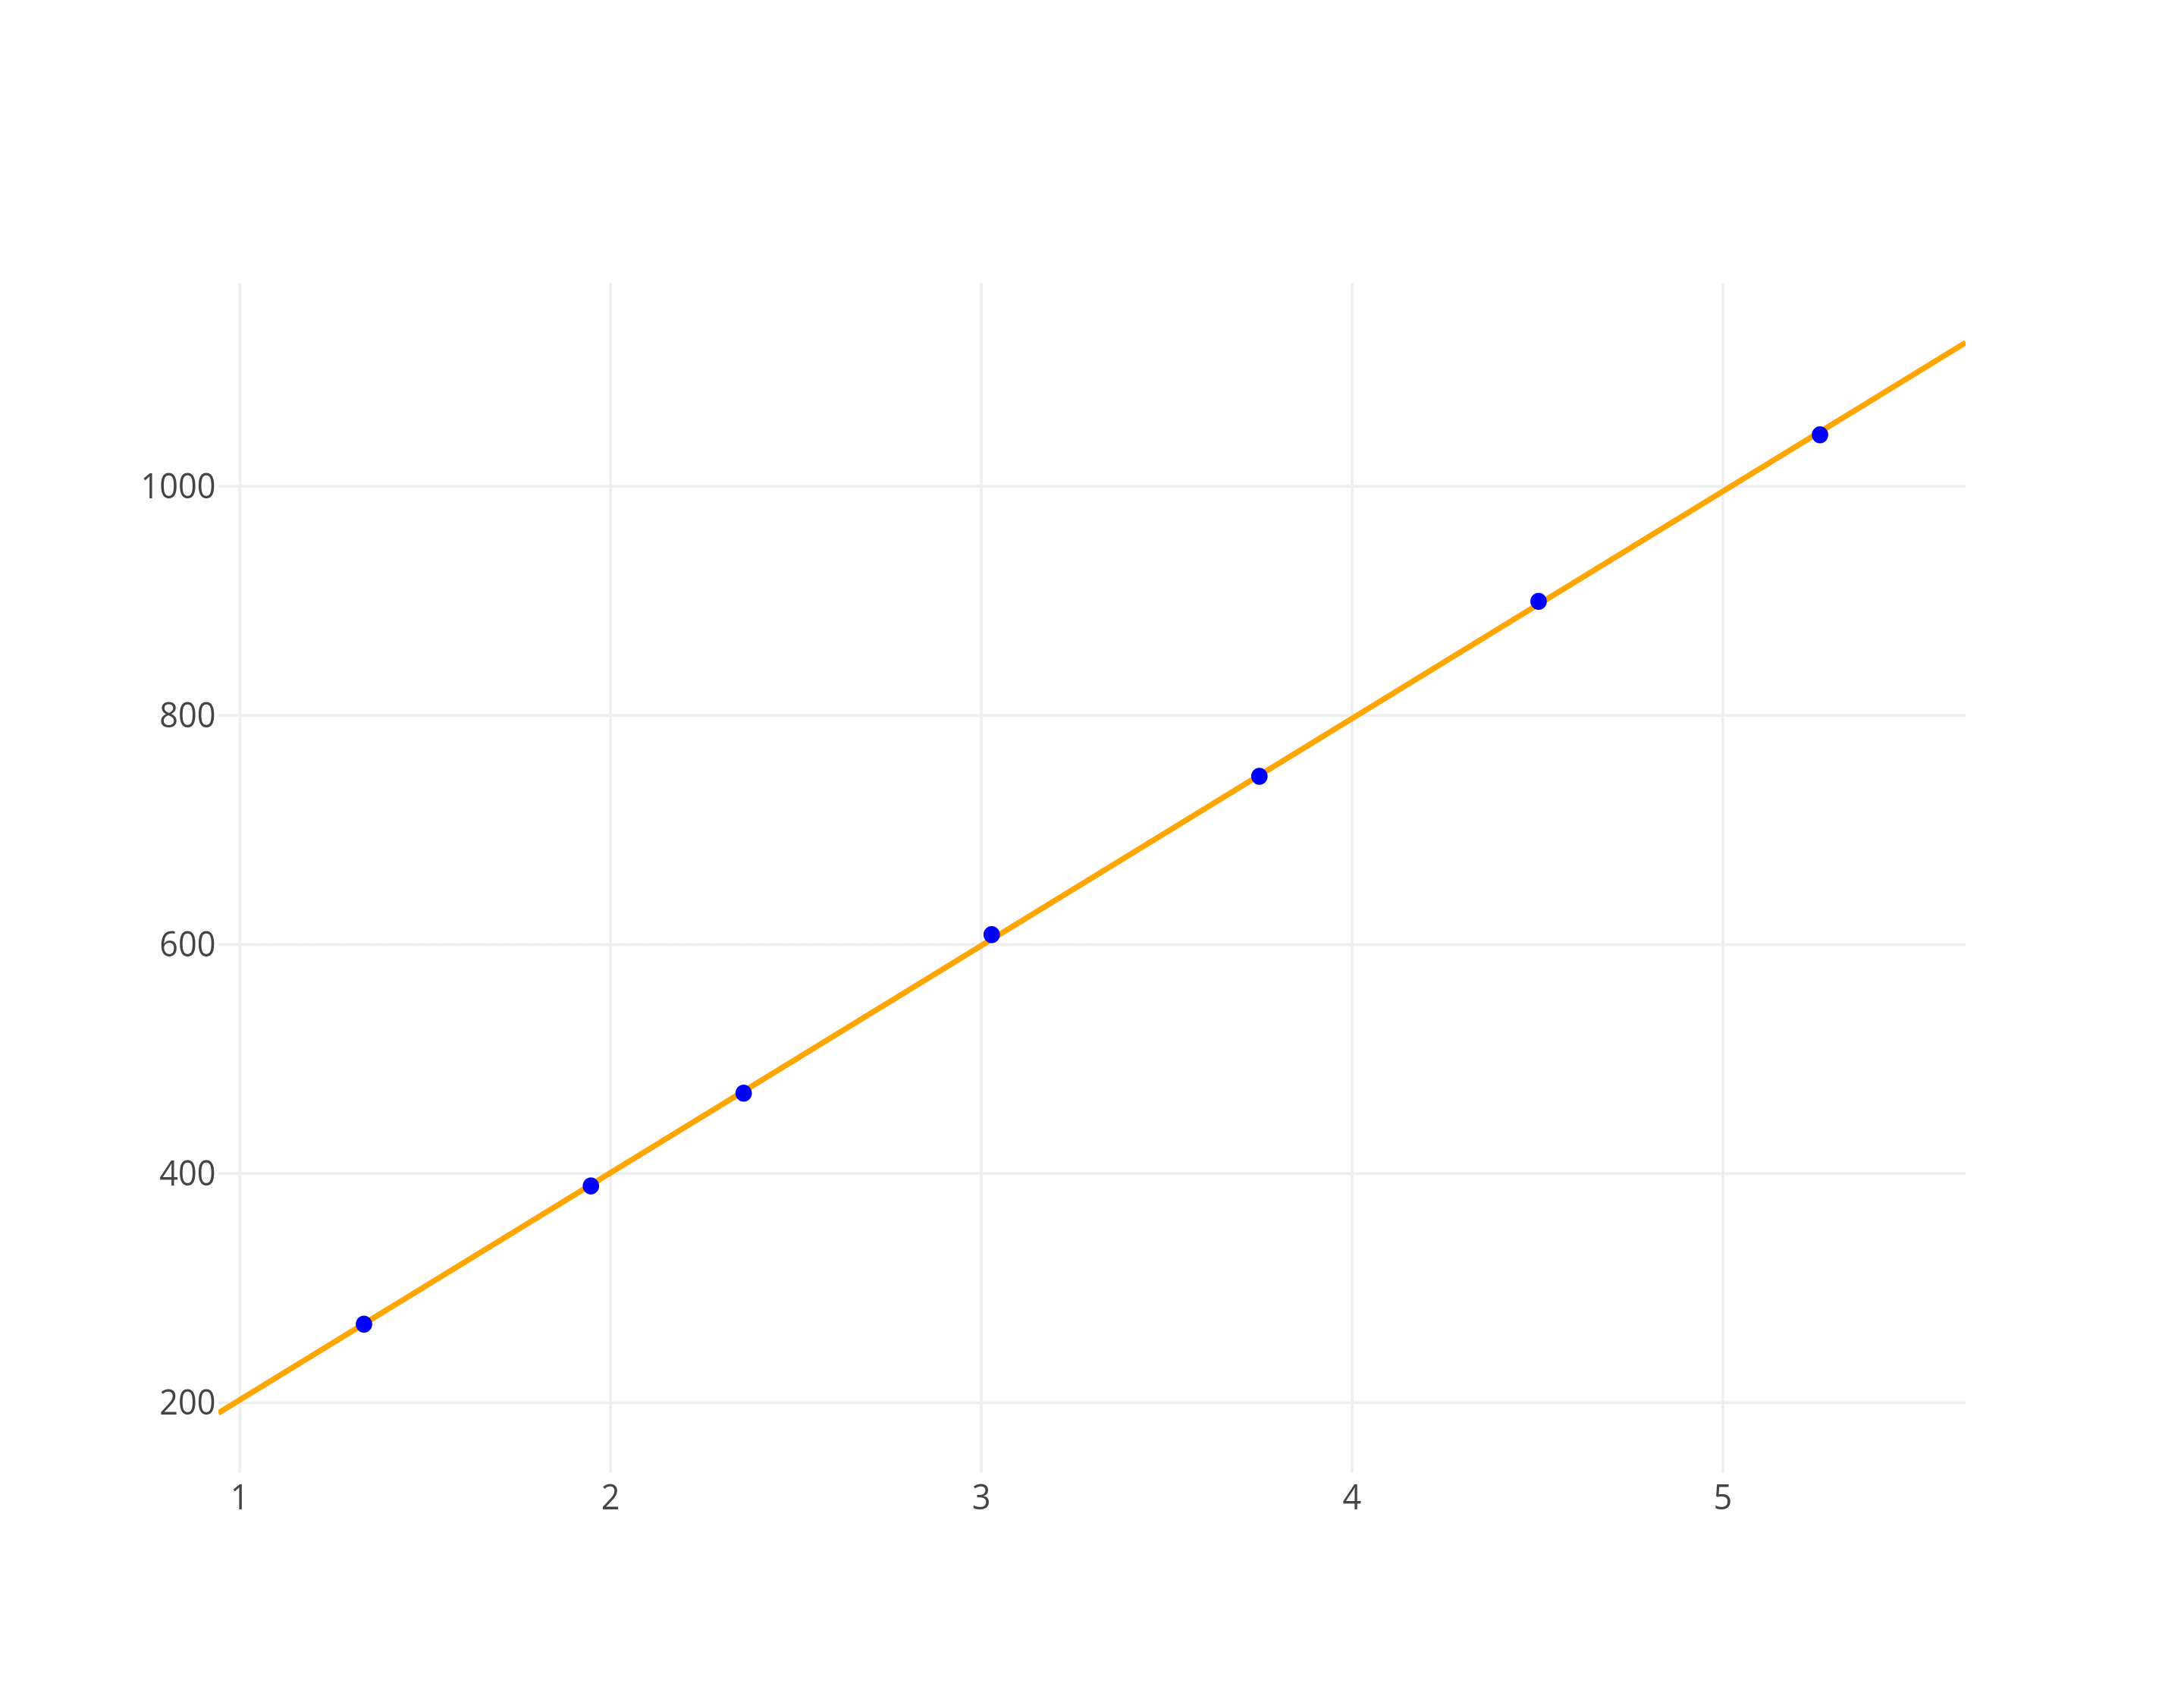
\includegraphics[scale=0.112]{PIC_3.png}
		\\\textbf{Рис. 3:} График зависимости $N(\Delta T)$
	\end{center}
	
	$$\gamma_1 = 198 \pm 5\ \text{мВт}/\text{К}$$
	
	\newpage
	
	%Страница 5
	
	\begin{flushleft}
		\footnotesize{Измерение удельной теплоемкости воздуха при постоянном давлении} \hspace{\fill} \footnotesize{5}
		\\[-0.3cm]\noindent\rule{\textwidth}{0.3pt}
	\end{flushleft}
	
	\paragraph{Определение удельной теплоемкости} \hfill
	
	Константа $\alpha$ остается постоянной в ходе обоих опытов, поэтому получим следующее выражение для удельной теплоемкости:
	$$c_p = \sfrac{\gamma_1 - \gamma_2}{\mu_1 - \mu_2} = (1.04 \pm 0.02)\ \sfrac{\text{кДж}}{\text{кг}\cdot\text{К}}$$
	где $\mu$ - массовые расходы воздуха.
	
	\paragraph{Определение доли тепловых потерь} \hfill
	
	Определим доли тепловых потерь относительно общей подводимой мощности, и запишем их в таблицу. В первой паре строк первый опыт, а во второй -- второй.
	
	\begin{center}
		\begin{tabular}{|c|c|c|c|c|c|c|c|}
			\hline
			$\Delta T$, К & $0.934$ & $1.720$ & $2.211$ & $2.629$ & $3.047$ & $3.612$ & $4.693$
			\\\hline
			$N_{\text{пот}}/N \cdot 10^2$ & $28.3 \pm 3.1$ & $24.5 \pm 2.1$ & $21.3 \pm 1.9$ & $25.4 \pm 1.8$ & $24.4 \pm 1.7$ & $26.8 \pm 1.6$ & $24.9 \pm 1.7$
			\\\hline
			$\Delta T$, К & $1.335$ & $1.947$ & $2.359$ & $3.028$ & $3.750$ & $4.503$ & $5.262$
			\\\hline
			$N_{\text{пот}}/N \cdot 10^2$ & $30.2 \pm 2.4$ & $29.9 \pm 1.9$ & $29.7 \pm 1.8$ & $30.3 \pm 1.6$ & $29.6 \pm 1.6$ & $29.8 \pm 1.5$ & $29.4 \pm 1.5$
			\\\hline
		\end{tabular}
		\textbf{Табл. 6:} Определение доли тепловых потерь
	\end{center}

	Поскольку при повышении температуры доля тепловых потерь также возрастает, судя по таблице, примерно равномерно, усредним эти величины для обоих опытов:
	$$\overline{\lambda_1} = \sfrac{N_{\text{пот}}}{N} \cdot 10^2 = (25.1 \pm 1.9)\%\ \ \ \ \ \ \ \ \ \ \ \ \ \ \ \ \ \ \overline{\lambda_2} = \sfrac{N_{\text{пот}}}{N} \cdot 10^2 = (29.8 \pm 1.8)\%$$
	
	\section{Выводы}
	В результате работы получено значение удельной теплоемкости воздуха при постоянном давлении
	$$c_p = (1.04 \pm 0.02)\ \sfrac{\text{кДж}}{\text{кг}\cdot\text{К}}$$
	что близко к табличному значению $c_{p\,0} = 1.005 \ \frac{\text{кДж}}{\text{кг}\cdot\text{К}}$ -- совпадения в пределах величины погрешности не вышло, но отклонение не превосходит двух величин погрешности. К возможным причинам такой ошибки можно отнести неточности измерений (флуктуации значения напряжения на милливольтметре) и нарушение проведения эксперимента, к примеру, в аудитории открывалось окно.
	
	Также в ходе работы определена доля тепловых потерь засчет теплового потока через стенки сосуда, а не непосредственно уносимого воздухом, прокачиваемым через сосуд. Доля колеблется между 25-30\%.
\end{document}